\documentclass[10pt,a4paper]{article}
\usepackage[utf8]{inputenc}
\usepackage{amsmath}
\usepackage{amsfonts}
\usepackage{amssymb}
\usepackage{german}
\usepackage{fancyhdr}
\usepackage{graphicx}
\usepackage{geometry}
\usepackage{color}
\usepackage[usenames,dvipsnames]{xcolor}
\usepackage{DejaVuSans}
\usepackage[T1]{fontenc}
\renewcommand*{\familydefault}{\sfdefault}
\geometry{verbose,a4paper,tmargin=35mm,bmargin=35mm,lmargin=25mm,rmargin=25mm}
\author{Dominik Heeb}
\title{Projektplan Semesterarbeit}
\pagestyle{fancy}
\fancyhead{}
\fancyhead[L]{Study stfld - Dynamic Parallel Checker}
\fancyhead[R]{Domink Heeb}
\fancyfoot{}
\fancyfoot[R]{Seite \thepage}
\begin{document}
\begin{titlepage}
	\begin{Huge}
		\begin{center}
				Study stfld \\Dynamic Parallel Checker\\[2.0cm]
		\end{center}
	\end{Huge}
	
	\begin{center}
		\begin{Large}
				by Dominik Heeb\\[1.0cm]
		\end{Large}
	\end{center}
\end{titlepage}

\newpage
\tableofcontents 
\newpage

\section{Problem stfld}
\begin{flushleft}
Im IL Code wird um ein Feld auf einem Objekt zu speichern ein Befehl namens stfld verwendet.
stfld arbeitet folgendermassen mit dem Stack:  \\
\begin{center}\begin{Large}
obj, value $\rightarrow$ ...
\end{Large}\end{center}
Für die Verarbeitung des Dynamic Parallel Checkers ist nötig and die Variable obj zu kommen.
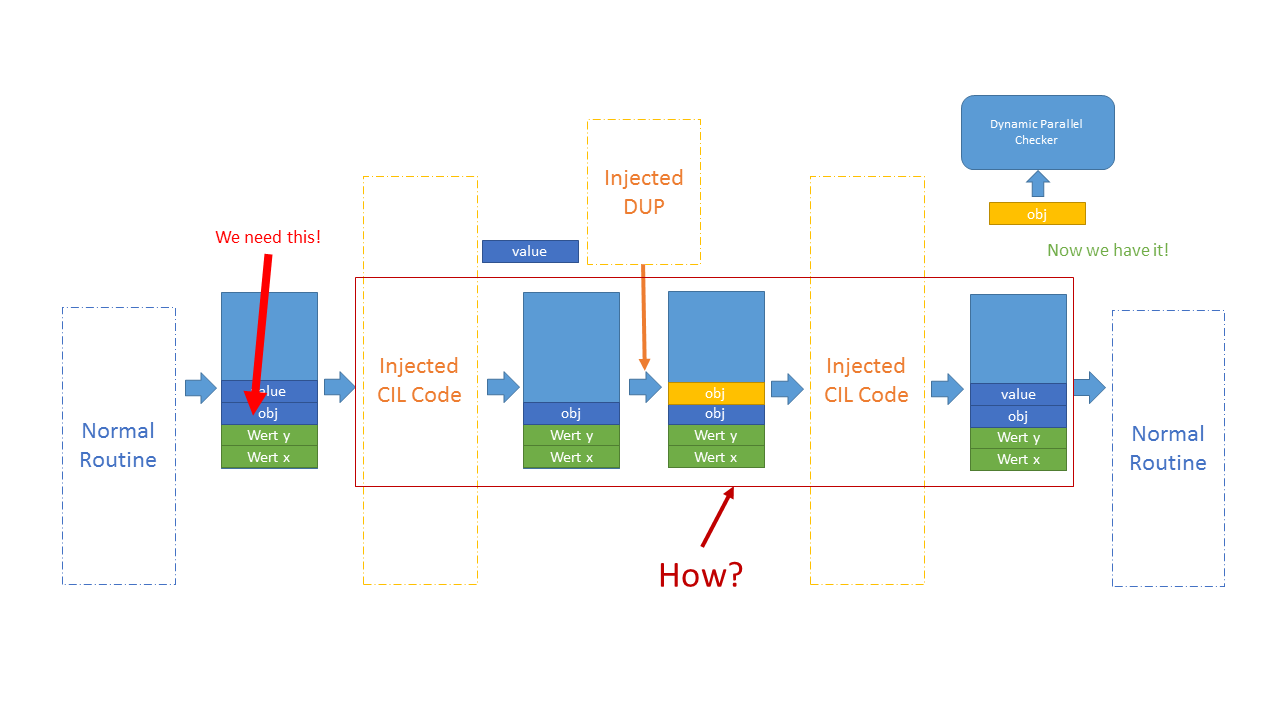
\includegraphics[width=16cm,height=7.5cm,trim=10mm 10mm 0mm 20mm, clip]{pictures/StudyStfld.png}
\end{flushleft}
\section{Lösungsmöglichkeiten}\label{sec:Lösungsmöglichkeiten}
\begin{flushleft}
Für die Lösung dieses Problems, gibt es verschiedene Wege:
\begin{enumerate}
\item Mittels lokaler Variablen, kann der Stack abgebaut und der Wert in eine lokale Variable gespeichert werden. Dieser Weg ist sehr Perfomant aber gefährlich bei Injection. Denn es besteht die Möglichkeit, dass eine vorgehend und nachfolgende Instruktion abhängig ist von einer lokalen Variable. Dies kann zu Fehlern führen.
\item Der Befehl call erlaubt das Aufrufen einer Funktion. Dabei werden Parameter abgebaut und nach dem Aufruf der Return Value wieder auf den Stack gelegt. Diese Möglichkeit erlaubt sicheres Aufbauen und abbauen des Stack. Es ist jedoch nur die Rückgabe eines Wertes möglich
\end{enumerate}
\end{flushleft}
\newpage
\section{Implementation}
\begin{flushleft}
Unter Kapitel \ref{sec:Lösungsmöglichkeiten} wurden die Möglichkeiten zur Lösung des Problems beschrieben. Bei der Implementation wurde Variante 1 gewählt, aber abgesichert, dass die Variable nicht genutzt wird. Diese Absicherung wird erreicht in dem eine neue lokale Variable innerhalb der Methode deklariert wird. In dieser kann der Top-Of-Stack Wert gespeichert und nach der Verarbeitung wieder auf den Stack geladen werden.
\includegraphics[width=16cm, clip]{pictures/Stackinjection.png}
Dieses Verfahren erlaubt es auf tiefere Werte als den Top-Of-Stack zuzugreifen und kann auf beliebige Grösse skaliert werden.
\end{flushleft}
\end{document}